\section{Direkte Fernlokalisierung mit Long Range}
\label{ch:phase4}
Für die direkte Fernlokalisierung mit \emph{Long Range} (LoRa) werden dedizierte Basisstationen eingesetzt. 
Die Kommunikation zwischen Basisstation und Ortungsdienst kann durch ein LAN- oder WLAN-Netzwerk gewährleistet werden.
Die Basisstationen bestimmen den \emph{Received Signal Strength Indicator} (RSSI) eingehender Übertragungen der mobilen Enheiten und übermitteln die gemessenen Werte dann an den Ortungsdienst.
Der Ortungsdienst kann mit den gesammelten Werten die Position der mobilen Einheit berechnen.

\subsection{RFM95}
\label{ch:hardwarechanges:sec:rfm95}
Bei dem \emph{RFM95} handelt es sich um ein LoRa-fähiges Radio-Modul für den Frequenzbereich 868/915 MHz \cite{hope2006rfm}. 
915 MHz sind jedoch nur in Amerika lizenzfrei, in Deutschland muss das Radio mit 868 MHz betrieben werden.

Für die Entwicklung wird das Modul auf einem Adafruit Feather M0 \emph{RFM95} LoRa Radio verwendet.
Dieses verwendet einen M0 Mikrocontroller zur Steuerung, einen Lithium-Akku-Ladeschaltkreis und einen Spannungswandler.
Zusätzlich ist eine Antenne notwendig. 
Die verwendete Antenne kann dabei einen große Unterschiede in der Reichweite verursachen, deshalb sollte eine Antenne für 868 MHz verwendet werden.
Da jedoch eine feste Antenne die mobile Einheit unhandlich machen würde, wird für diese eine Kabelantenne verwendet, diese hat die Länge einer halben Wellenlänge (17,3 cm).

Abbildung \ref{fig:lorafeather} zeigt ein Adafruit Feather M0 \emph{RFM95} LoRa Radio. 
Für die Basisstation wird ein Feather M0 \emph{RFM95} LoRa Radio mit fester Antenne verwendet.

\begin{figure}[h]
  \centering
	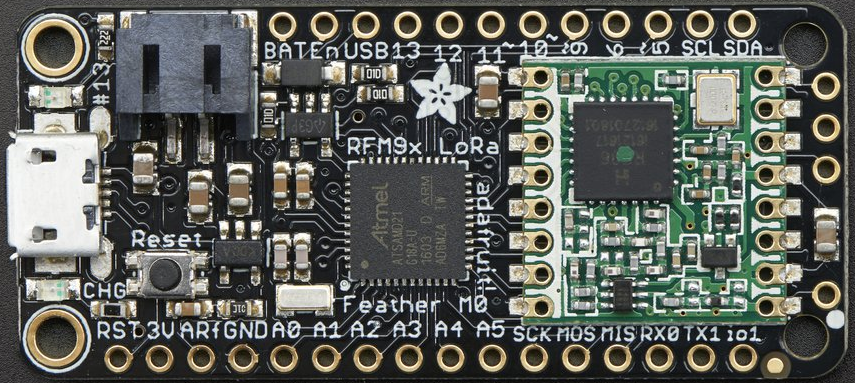
\includegraphics[width=\textwidth]{images/loraada.png}
  \caption{Adafruit Feather M0 \emph{RFM95} LoRa Radio. Bild von Adafruit Industries\protect \footnotemark.}
  \label{fig:lorafeather}
\end{figure}
\footnotetext{\url{https://www.adafruit.com/product/3178}}

\subsubsection{RadioHead RFM9x für Arduino}
Der M0 Mikrocontroller ist Arduino kompatibel, wird zusätzlich die \emph{RadioHead RFM9x} Bibliothek verwendet, kann er über ein \emph{SPI Interface} das Radio steuern.
Adafruit stellt dazu eine englischsprachige Anleitung zur Verfügung\footnote{\url{https://learn.adafruit.com/adafruit-feather-m0-radio-with-lora-radio-module/setup}}.
Es wird die \emph{RadioHead RFM9x} Bibliothek Version 1.62 verwendet.

\subsection{Reichweite von LoRa}
Die Versuche mit LoRa wurden an einer anderen Tunnelbaustelle durchgeführt.
An der Tunnelbaustelle Ulm wird mit Sprengungen vorgetrieben.
Nach der Sprengung wird der Tunnel mit Spritzbeton ausgekleidet und danach wird in drei Schritten geschalt. 
Im ersten Schritt wird ein Filz und eine Folie gegen das Eindringen von Wasser eingebracht, danach folgt die Bewehrung und abschließend wird die Bewehrung einbetoniert.
Für jeden Schritt wird ein stählerner Schalungswagen verwendet, folglich sind drei stählerne Hindernisse im Tunnel, die Signale absorbieren.
Abbildung \ref{fig:schalungswagen} zeigt einen der Schalungswagen, der als Hindernis gedient hat.

\begin{figure}[h]
  \centering
	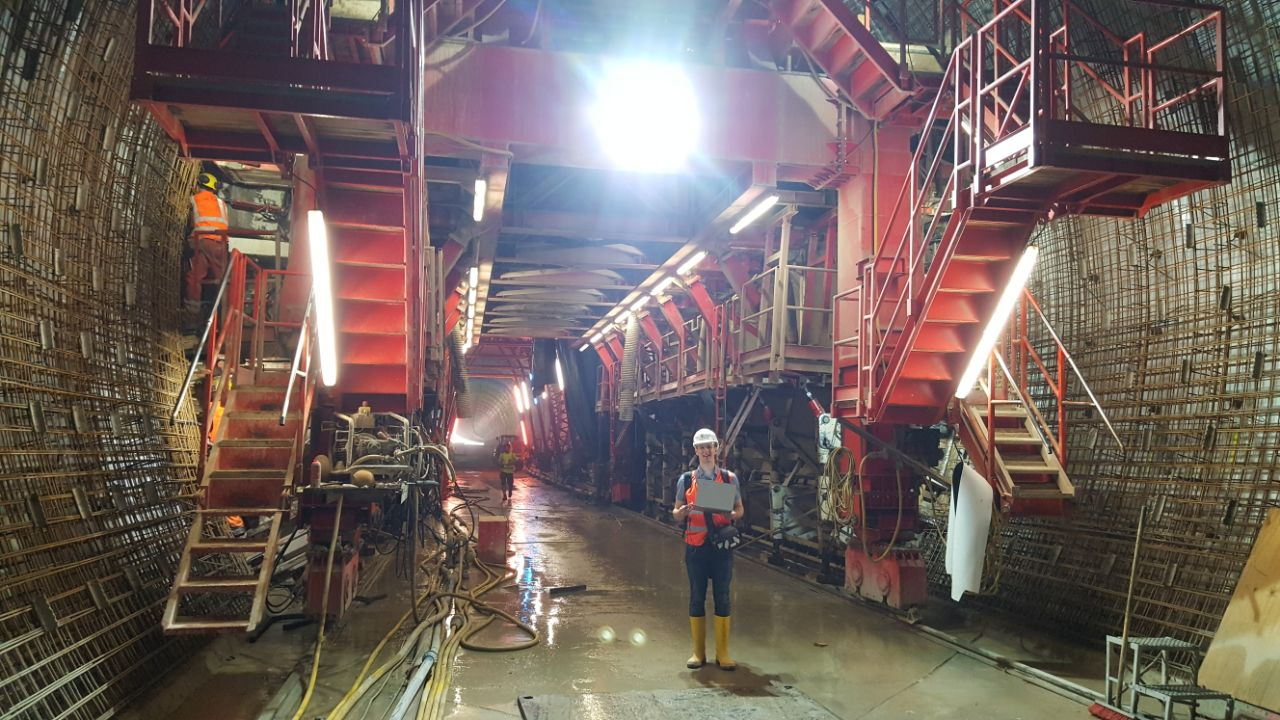
\includegraphics[width=\textwidth]{images/schalungswagen.jpg}
  \caption{Schalungswagen für das Betonieren im Tunnel Ulm.}
  \label{fig:schalungswagen}
\end{figure}

\subsubsection{Methodik} 
Die Reichweite wurde für zwei Situationen bestimmt.
Zum einen durch einen Schalungswagen und dann durch den freien Tunnel, zum anderen durch alle drei Schalungswagen für eine Situation mit maximaler Abschirmung durch die Hindernisse.
Die zwei Messtrecken werden in Abbildung \ref{fig:rangelora} skizziert.

\begin{figure}[h!]
  \centering
	\includegraphics[width=\textwidth]{images/rangelora.eps}
  \caption{Messtrecken zur Festellung der Reichweite von LoRa.}
  \label{fig:rangelora}
\end{figure}

Die mobile Einheit wurde jeweils direkt an der Bewehrung platziert und es wurde auf der selben Seite gelaufen, damit die Abschirmung durch die Schalungswagen maximal ist.
Danach wurde die Basisstation immer weiter entfernt, bis keine Pakete der mobilen Einheit mehr empfangen werden konnten.
Abbildung \ref{fig:lorabasis} zeigt die Platzierung der mobilen Einheit an der Bewehrung.
Erneut konnte die Plastikbox aufgrund des Versuchsaufbaus nicht geschlossen werden.

Die mobile Einheit wurde als "`außer Reichweite"' angesehen, wenn versendete Pakete der mobilen Einheit nicht mehr bei der Basisstation ankamen.
Durch das Entfernen des körperlichen Hindernisses war es möglich wieder eine Verbindung herzustellen.
Es wurde sowohl mit einer Sendeleistung von 5 dBm für einen geringen Sendeverbrauch als auch mit 23 dBm Sendeleistung für maximale Reichweite gemessen.
Die Messungen werden in 12,5 m Abständen angegeben, da in diesem Tunnel die Länge eines Schalungselements 12,5 m beträgt.
Es werden, wie in Abschnitt \ref{ch:hardwarechanges:sec:rfm95} besprochen, zwei unterscheidliche Typen von Antennen verwendet. 
Während die Basisstation eine feste Antenne aufweist, verwendet die mobile Einheit eine Kabelantenne entsprechend der halben Wellenlänge. 

\begin{figure}[h]
  \centering
	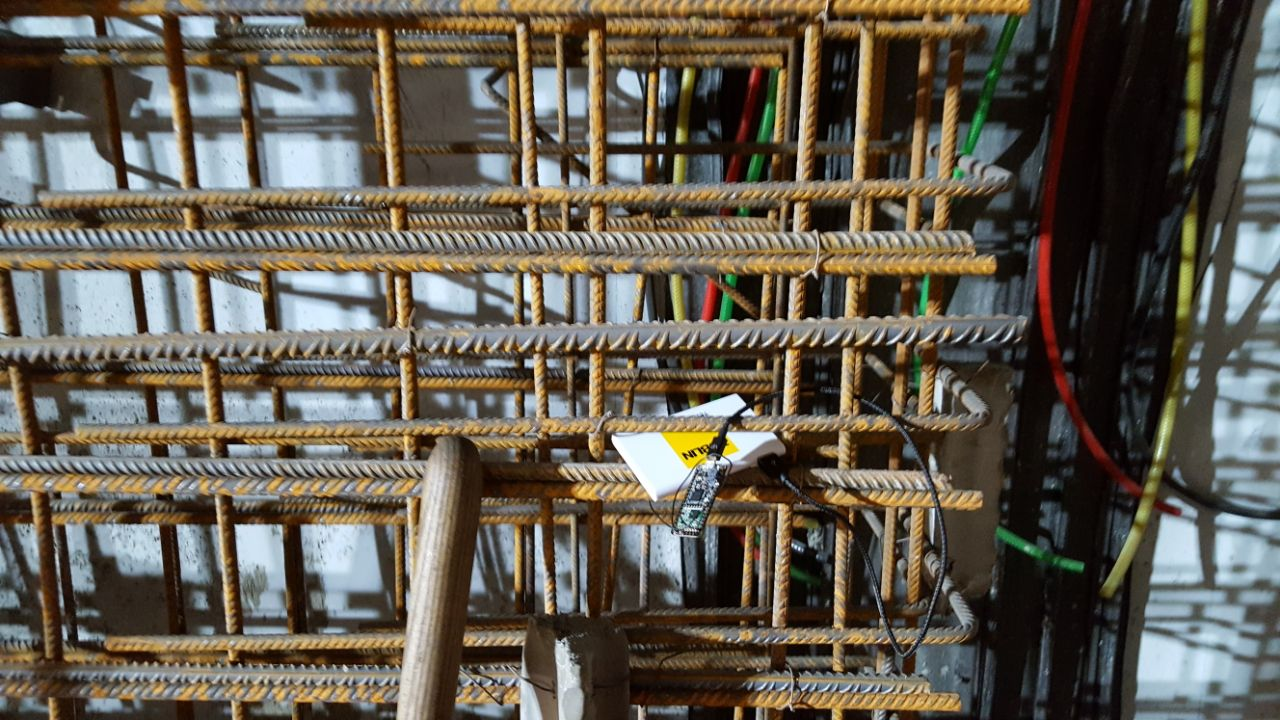
\includegraphics[width=\textwidth]{images/lorabasis.jpg}
  \caption{Platzierung der mobilen Einheit an der Bewehrung des Tunnels.}
  \label{fig:lorabasis}
\end{figure}

\subsubsection{Ergebnisse}
Tabelle \ref{table:rangelora} zeigt die Ergebnisse für das \emph{RFM95}.
Da das lose Auflegen des Deckels der Plastikbox zu keiner Veränderung bei der Reichweite führte gibt die Tabelle nur Werte für den offenen Aufbau an. 
Der Test mit 23 dBm Sendeleistung durch alle drei Schalungswagen musste nach 350 m abgebrochen werden, weil ein weiterkommen nicht möglich war.
Da jedoch für diese Sendeleistung bereits nach circa 250 m die Varianz des RSSI den Zusammenhang zwischen Distanz und RSSI überwiegt, kann die tatsächliche Reichweite dieser Sendeleistung nicht ausgenutzt werden.
Für eine sichere Erkennung des 250-Meter-Abschnitts müsste daher alle 500 m eine Basisstation aufgestellt werden.

\begin{table}[h]
	\centering
	\caption{Sendereichweite LoRa-basierter mobiler Einheiten}
	\label{table:rangelora}
	\begin{tabular}{p{2.2cm}|p{1.5cm}|R{2.5cm}|p{3.5cm}|R{3cm}}
		Verwendetes Modul & Aufbau & Sendeleistung & Strecke & Maximale Sendereichweite \\
		\hline
		\emph{RFM95} & Offen & 5 dBm & Wenige Hindernisse & 250 m \\
		\emph{RFM95} & Offen & 5 dBm & Viele Hindernisse & 100 m \\
		\hline
		\emph{RFM95} & Offen & 23 dBm & Wenige Hindernisse & 1250 m \\
		\emph{RFM95} & Offen & 23 dBm & Viele Hindernisse & >350 m \\
	\end{tabular}
\end{table}

\subsubsection{Bewertung}
LoRa entfaltet im Tunnel eine sehr hohe Reichweite und es kann eine lückenlose Überwachung von Personen durchgeführt werden.
Voll nutzen lässt sich die Reichweite jedoch nicht, da die Varianz des RSSI den Zusammenhang zwischen Distanz und RSSI schon nach circa 250 m überwiegt. 
Hingegen führt eine starke Reduktion der Sendeleistung zu einer mangelnder Penetration von Hindernissen.
Daher sollte ein Kompromiss der Sendeleistung geschlossen werden. 
Eine Sendeleistung von 10 dBm sollte eine ausreichende Reichweite im Szenario mit vielen Hindernissen bieten.
Alternativ kann die mobile Einheit auch ein \emph{Send-Receive-Schema} umsetzen und von der Basisstation eine dynamisch angepasste Sendeleistung empfangen, die sich nach der Menge der Hindernisse richtet.

Wird die Sendeleistung dynamisch so festgelegt, dass eine Reichweite von 250 Metern erreicht wird, benötigt ein Mitarbeiter bei 30 km/h 30 Sekunden, um sie zu durchqueren.
Eine derart lange Intervallzeit würde jedoch dazu führen, dass eine volle Minute ohne Aktualisierung der Position vergeht, sollte ein Paket verloren gehen.
Das Sendeintervall wird deshalb auf 10 Sekunden gesetzt.

\subsection{LoRa-Implementierung}
Die Implementierung für die Lokalisierung mit LoRa ist sehr simpel.
Die mobile Einheit versendet regelmäßig ein Paket, welches einen Identifikator für die mobile Einheit enthält.
Das Sendeintervall beträgt entsprechend der hohen Reichweite 10 Sekunden.

Die Basisstation empfängt durchgehend und bestimmt den RSSI für eingehende Pakete.
Anschließend leitet sie den Identifikator der mobilen Einheit zusammen mit dem RSSI und einer Kennung für die Basisstation an den Ortungsdienst weiter.

Auf der mobilen Einheit müssen lediglich die Sendefrequenz, die Sendeleistung und der Identifikator gesetzt werden, dann kann immer nach Ablauf des Sendeintervalls gesendet werden.
Die Basisstation muss dabei auf der selben Frequenz aktiv sein und empfangen.


\subsection{Untersuchung des Stromverbrauchs}
Der Stromverbrauch soll mit dem INA219 genauer bestimmt werden, der INA219 und die verwendete Methodik werden in Abschnitt \ref{ch:phase1:sec:energie} beschrieben.

\subsubsection{Theoretische Stromverbrauchsabschätzung}
Für die Berechnung des theroretischen Verbrauchs der mobilen Einheit werden die Datenblätter des M0 Mikrocontrollers und des \emph{RFM95} Radios herangezogen. 
Die dort gelisteten Verbräuche sind in Tabelle \ref{table:m0power} und Tabelle \ref{table:lorapower} zu finden.

\begin{table}[h]
  \centering
  \caption{Stromverbrauch des M0 Mikrocontrollers, aus \cite{nxp2016m0}}
	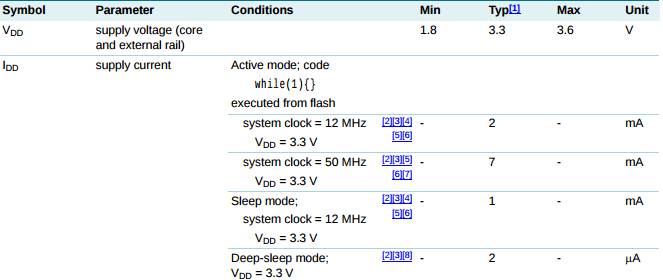
\includegraphics[width=\textwidth]{images/m0power.png}
  \label{table:m0power}
\end{table}

\begin{table}[h]
  \centering
  \caption{Stromverbrauch des \emph{RFM95}, aus \cite{hope2006rfm}}
	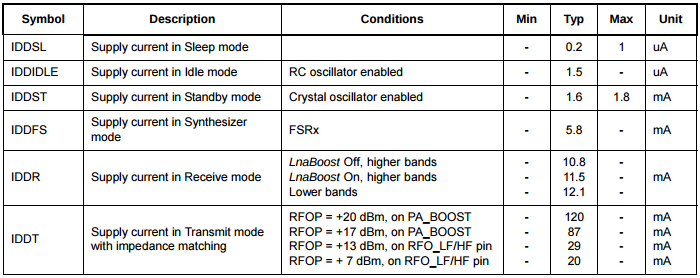
\includegraphics[width=\textwidth]{images/lorapower.png}
  \label{table:lorapower}
\end{table}

Da das Adadfruit Feather M0 \emph{RFM95} Lora Radio sich nur durch die Ersetzung des \emph{CP2014} durch den \emph{Cortex-M0} zum Adafruit Feather \emph{nRF52} unterscheidet werden die 155 \textmu A für die sonstigen Komponenten übernommen.

Die Sendeleistung des \emph{RFM95} Radio ist zwischen 5 dBm und 23 dBm einstellbar. 
Das Datenblatt listet jedoch nur Verbräuche zwischen 7 dBm und 20 dBm Sendeleistung, der Verbrauch wird für diese beiden Sendeleistungen berechnet.
Für die Nachricht "`TagTest"' werden 20 Bytes (160 Bits) versendet, es wird angenommen, dass zuvor 500 Bits für die Kollisionskontrolle belauscht werden.
Für die restliche Zeit wird angenommen, dass sich der \emph{M0} Mikrocontroller im \emph{Deep-sleep mode} und das \emph{RFM95} Radio im \emph{IDDIDLE} Modus befindet.
Damit ergibt sich ein durchschnittlicher Verbrauch $y$ in Höhe von: 

$y = \frac{1}{10} * [(10 - \frac{Bits\_gesendet}{21875 b/s} - \frac{Bits\_empfangen}{21875 b/s}) * (M0\_Deep\_sleep\_mode + RMF95\_IDDIDLE + 155 {\mu}A) + \frac{Bits\_gesendet}{21875 b/s} * RFM95\_XdBm + \frac{Bits\_empfangen}{21875 b/s} * RFM95\_IDDR]$

Für die folgende Rechnung wird eine Sendeleistung von 20 dBm angenommen:

$y_{20dBm} = \frac{1}{10} * [(10s - 0,0073s - 0,0229s) * 0,1585mA + 0,0073s * 120mA + 0,0229s * 12,1mA]$\\[0.5cm]
$y_{20dBm} \approx \frac{1}{10} * (1,58mA + 0,876mA + 0,2771mA) = 0,2683mA$

Als Stromsparmaßnahme wird für die folgende Rechnung die Sendeleistung auf 7 dBm reduziert:

$y_{7dBm} = \frac{1}{10} * [(10s - 0,0073s - 0,0229s) * 0,1585mA + 0,0073s * 20mA + 0,0229s * 12,1mA]$\\[0.5cm]
$y_{7dBm} \approx \frac{1}{10} * (1,58mA + 0,146mA + 0,2771mA) = 0,1953mA$

\subsubsection{Tatsächlicher Stromverbrauch von LoRa}
\label{ch:phase3:sec:powerlora}
Der Stromverbrauch der Implementierung mit LoRa wurde mit 5 dBm und 23 dBm Sendeleistung überprüft.
Abbildung \ref{fig:lora5} zeigt den Lastverlauf für den Start einer mobilen Einheit mit LoRa bei 5 dBm.

Nach einer circa 3-sekündigen Startphase wechselt der LoRa Feather in den regulären Betrieb, er sollte dann immer nach 10 Sekunden Ruhezustand senden.
Dieser jedoch vom Zeitgeber nicht ganz eingehalten, die mobile Einheit befindet sich zwischen den Sendevorgängen circa 11 Sekunden im Ruhezustand, dies sollte bei der Implementierung beachtet werden.
Im Ruhezustand liegt der Verbrauch des LoRa Feather bei 0,9 bis 1,0 mA, beim Senden unterscheiden sich die Vebräuche je nach Sendeleistung deutlich.

\begin{figure}[h!]
  \centering
	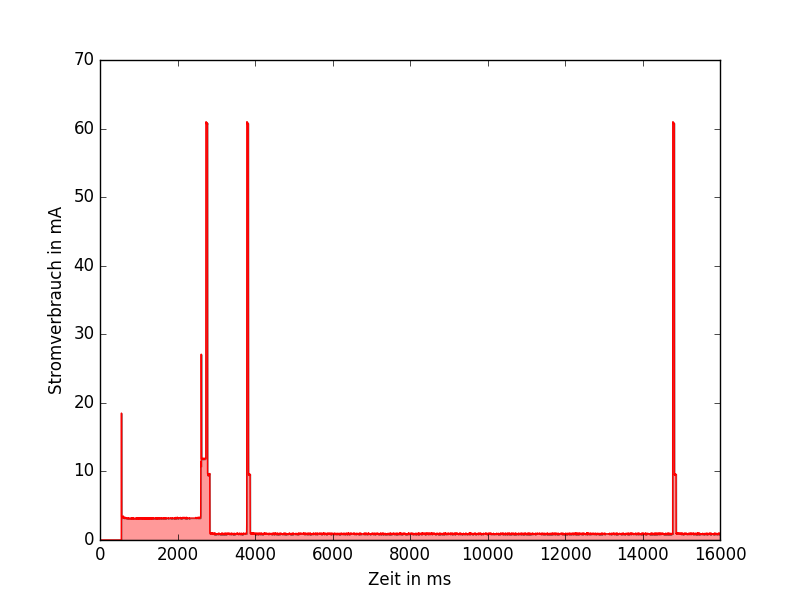
\includegraphics[width=\textwidth]{plots/lora5.png}
  \caption{Stromverbrauchskurve einer Implementierung mit LoRa.}
  \label{fig:lora5}
\end{figure}

Die Abbildung \ref{fig:lora235send} zeigt die Sendeverbräuche für eine Sendeleistung von 23 dBm in Rot und für 5 dBm in Grün.
Gut zu erkennen ist hier auch, dass ein Sendevorgang bei LoRa deutlich länger als bei BLE dauert, obwohl vergleichbar viele Bits übertragen werden.

\begin{figure}[h!]
  \centering
	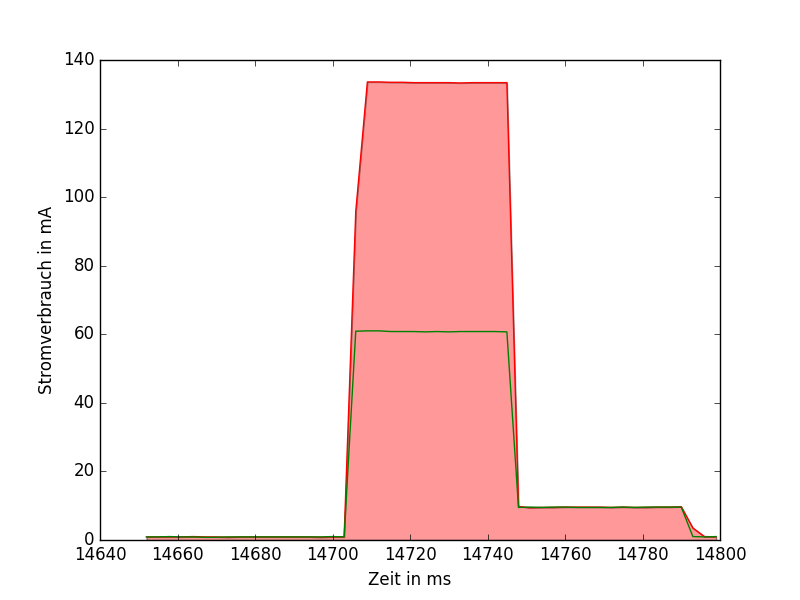
\includegraphics[width=\textwidth]{plots/lora235send.png}
  \caption{Stromverbrauchskurve eines Ortungsvorgangs mit LoRa.}
  \label{fig:lora235send}
\end{figure}

Die Ergebnisse der Messungen sind in Tabelle \ref{table:lora235ina} gelistet.
Für den \emph{RFM95} Feather liegt der Ruheverbrauch deutlich niedriger, da jedoch die selben Schaltungen für Akku-Ladung und Spannungsregelung zum Einsatz kommen, scheint der \emph{CP2104}, welcher zum Programmieren des \emph{ESP8266} beziehungsweise \emph{nRF52} dient, mindestens 6 mA zu verbrauchen.
Für den normalisierten Stromverbrauch wurde der Verbrauch im Ruhezustand subtrahiert. 
Dies beschränkt den Verbrauch auf den für die tatsächliche Funktion nötigen Anteil.

\begin{table}[h!]
	\centering
	\caption{Stromverbrauch mobiler Einheiten mit LoRa}
	\label{table:lora235ina}
	\begin{tabular}{l|l|R{2.5cm}|R{2cm}}
		Hardware & Programm & $\varnothing$ Verbrauch in mA (normalisiert) & Laufzeit in Stunden\\
		\hline
		LoRa Feather & LoRa 23 dBm Sendeleistung & 1,47 (0,57) & 952,4\\
		LoRa Feather & LoRa 5 dBm Sendeleistung & 1,20 (0,30) & 1166,7\\
	\end{tabular}
\end{table}






\section{Zusammenfassung}
Die folgenden Abschnitte sollen die Ergebnisse des Kapitels zusammenfassen und aufarbeiten.

\subsection{Reichweite}
Die Zuverlässigkeit bei der Erkennung von Bereichswechseln hängt maßgeblich von der Reichweite der Funktechnologie und der Länge des Sendeintervalls ab.
Tabelle \ref{table:ranges} fasst die Ergebnisse der Versuche zur Reichweite zusammen. 
Es wurden jeweils Ergebnisse ohne Gehäuse ausgewählt, da die Reichweite durch ein Gehäuse nur im Falle des \emph{ESP-12S} zu einer Verringerung der Reichweite geführt hat. 
Die Ergebnisse des \emph{ESP-12S} sind jedoch zugunsten des \emph{ESP-12F} nicht gelistet.

\begin{table}[h]
	\centering
	\caption{Sendereichweite mobiler Einheiten}
	\label{table:ranges}
	\begin{tabular}{l|l|l|R{3cm}}
		Protokoll & Verwendetes Modul & Strecke & Maximale Sendereichweite \\
		\hline
		IEEE 802.11b & \emph{ESP-12F} & Wenige Hindernisse & 88 m \\
		BLE 5.0 & \emph{nRF52} & Wenige Hindernisse & 32 m \\
		LoRa & \emph{RFM95} 5 dBm & Wenige Hindernisse & 250 m \\
		LoRa & \emph{RFM95} 23 dBm & Wenige Hindernisse & 1250 m \\
		\hline
		IEEE 802.11b & \emph{ESP-12F}  & Viele Hindernisse & 32 m \\
		BLE 5.0 & \emph{nRF52}  & Viele Hindernisse & 14 m \\
		LoRa & \emph{RFM95} 5 dBm & Viele Hindernisse & 100 m \\
		LoRa & \emph{RFM95} 23 dBm & Viele Hindernisse & >350 m \\
	\end{tabular}
\end{table}

Der Abstand der Basisstationen für die Bereichsortung ist mit 250 Metern gegeben. 
Die einzige Funktechnologie, die über 125 Meter im Tunnel erreichte, ist LoRa.
Sie ist deshalb die einzige getestete Funktechnologie, die eine lückenlose Ortung ermöglicht.
Zu beachten ist, dass LoRa keine Kollisionsvermeidung verwendet, stattdessen wird auf einem zufälligem Kanal gesendet.
Es muss davon ausgegangen werden, dass manche Nachrichten verloren gehen.
Das Sendeintervall sollte deshalb deshalb nur auf die Hälfte des gewünschten Ortungsintervalls gesetzt werden. 
Um das Problem durch redundantes Senden zu umgehen, wurde das Sendeintervall in dieser Arbeit auf 10 Sekunden gesetzt.

Bei BLE und IEEE 802.11 entscheidet die Reichweite über das Sendeintervall, da hier Versorungslücken bei der jeweiligen Funktechnologie entstehen.
Sie werden dabei so gesetzt, dass beim Durchqueren des abgedeckten Bereichs mit 30 km/h mehrfach gesendet wird.
In dieser Arbeit wurden die Sendeintervalle für IEEE 802.11 auf 5 Sekunden und für BLE auf eine Sekunde gesetzt.

Kürzere Sendeintervalle führen dabei zu einer höheren Erkennungszuverlässigkeit, längere Sendeintervalle senken den Stromverbrauch.

\subsection{Mobile Einheiten}
Im Laufe dieser Arbeit wurden mehrere mobile Einheiten implementiert, diese sind in Tabelle \ref{table:implemen} gelistet.

\begin{table}[h]
	\centering
	\caption{Implementierungen}
	\label{table:implemen}
	\begin{tabular}{l|l|p{2.5cm}|p{5.8cm}}
		Protokoll & Hardware & Art der Fernlokalisierung & Programm \\
		\hline
		IEEE 802.11 & \emph{ESP8266} & Indirekt & \emph{WiFi-LLS} \cite{chen2007design} \\
		IEEE 802.11 & \emph{ESP8266} & Indirekt & \emph{Assoziations-Lokalisierung} \\
		\hline
		IEEE 802.11 & \emph{ESP8266} & Direkt & \emph{RADAR} \cite{bahl2000radar} \\
		IEEE 802.11 & \emph{ESP8266} & Direkt & \emph{Probe-Request-Lokalisierung} \\
		\hline
		BLE & \emph{nRF52} & Direkt & Ortung mit \emph{Bluetooth-Low-Energy-Advertising} \cite{jianyong2014rssi} \\
		\hline
		LoRA & \emph{RFM95} & Direkt & Ortung mit LoRa RSSI \\
	\end{tabular}
\end{table}

Die Implementierungen \emph{Assoziations-Lokalisierung} und \emph{Probe-Request-Lokalisierung} sind dabei Verbesserungen gegenüber den in der Literatur vorgeschlagenen Implementierungen, um den Stromverbrauch der jeweiligen mobilen Einheit zu senken.
Bei \emph{Ortung mit LoRa RSSI} wurde entgegen der Literatur der RSSI als Messwert gewählt.
Die Konzepte der anderen Implementierungen entspringen der Literatur.

\subsection{Stromverbrauch}
Die Implementierungen wurden anschließend auf ihren Stromverbrauch untersucht.
Ausgewählte Ergebnisse sind in Tabelle \ref{table:consumptions} aufgelistet.
Für den normalisierten Stromverbrauch wurde der Verbrauch im Ruhezustand subtrahiert. 
Dies beschränkt den Verbrauch auf den für die tatsächliche Funktion nötigen Anteil.

\begin{table}[h]
	\centering
	\caption{Stromverbrauch mobiler Einheiten}
	\label{table:consumptions}
	\begin{tabular}{l|p{3.2cm}|p{5.5cm}|R{2.5cm}}
		Protokoll & Modul & Programm  & $\varnothing$ Verbrauch (normalisiert)\\
		\hline
		IEEE 802.11 & \emph{ESP8266} Feather & \emph{WiFi-LLS} & 42,20 (34,10)\\
		IEEE 802.11 & \emph{ESP-12F} & \emph{WiFi-LLS} & 36,50 (35,20)\\
		IEEE 802.11 & \emph{ESP8266} Feather & \emph{Assoziations-Lokalisierung} & 15,40 (7,30) \\
		IEEE 802.11 & \emph{ESP-12F} & \emph{Assoziations-Lokalisierung} & 8,80 (7,50)\\
		IEEE 802.11 & \emph{ESP-12F} & \emph{Assoziations-Lokalisierung} (kein \emph{Access Point} in Reichweite) & 17,10 (17,10)\\
		\hline
		IEEE 802.11 & \emph{ESP8266} Feather & \emph{RADAR} & 16,70 (8,60)\\
		IEEE 802.11 & \emph{ESP-12F} & \emph{RADAR} & 10,10 (8,80) \\
		IEEE 802.11 & \emph{ESP8266} Feather & \emph{Probe-Request-Lokalisierung} & 9,70 (2,70)\\
		IEEE 802.11 & \emph{ESP-12F} & \emph{Probe-Request-Lokalisierung} & 1,80 (1,80)\\
		\hline
		BLE & \emph{nRF52} Feather & Ortung mit \emph{BLE-Advertising} & 7,37 (0,04)\\
		\hline
		LoRa & \emph{RFM95} Feather & Ortung mit LoRa RSSI (5 dBm) & 1,20 (0,30)\\
		LoRa & \emph{RFM95} Feather & Ortung mit LoRa RSSI (23 dBm) & 1,47 (0,57)\\
	\end{tabular}
\end{table}

Zu erkennen ist, dass die umliegenden Komponenten der verwendeten Adafruit Feather einen hohen passiven Stromverbrauch verursachen.
Direkt gezeigt werden konnte dieser Effekt jedoch im Zuge dieser Arbeit nur für das \emph{ESP8266} Feather, da nur dort ein einzelnes Modul vorhanden war.

Außerdem wurde gezeigt, dass IEEE 802.11-basierte Lösungen, die einem Netzwerk beitreten mehr Strom verbrauchen als solche, die darauf verzichten.
Die Einsparungen der \emph{Probe-Request-Lokalisierung} resultieren aus tieferen Schlafzuständen und dem Verzicht auf das Empfangen von \emph{Beacons}.
Zusätzlich leiden IEEE 802.11-basierte Lösungen, die einem Netzwerk beitreten, an den besonderen Bedingungen im Tunnelbau.
Da in Arbeitsbereichen vor dem Tunnel keine Abdeckung durch ein WLAN-Netzwerk herrscht, sucht die mobile Einheit nach dem WLAN-Netzwerk.
Dieser Vorgang ist energetisch deutlich teurer als das Halten einer Verbindung zu einem Netzwerk.

Mittelt man den zusätzlichen Verbrauch der Komponenten des \emph{ESP8266} Feather und überträgt diese auf das \emph{nRF52} Feather, ist BLE beim Stromverbrauch den anderen Protokollen weit überlegen.
Die Sendevorgänge von BLE sind sehr kurz und verbrauchen vergleichsweise wenig Strom.

LoRa verbraucht mehr Strom als BLE, hat aber auch eine deutlich höhere Reichweite.
Es ordnet sich beim Verbrauch zwischen BLE und IEEE 802.11 ein, wobei der Ruheverbrauch von knapp 1 mA den Sendeverbrauch überwiegt. 
Die mobilen Einheiten mit 5 dBm und 23 dBm Sendeleistung liegen deshalb beim Verbrauch über eine Stunde recht nah beieinander.

Abbildung \ref{fig:alle} gibt einen Überblick über den Verbrauch der Implementierungen bei der Ortung. 
\emph{RADAR} wird nicht gezeigt, da es keine Vorteile gegenüber der \emph{Probe-Request-Lokalisierung} bietet und mehr Strom verbraucht.
Die \emph{Assoziations-Lokalisierung} wird nicht gezeigt, da hier die Ortung im Zuge des \emph{Join} stattfindet.

\begin{figure}[h!]
  \centering
	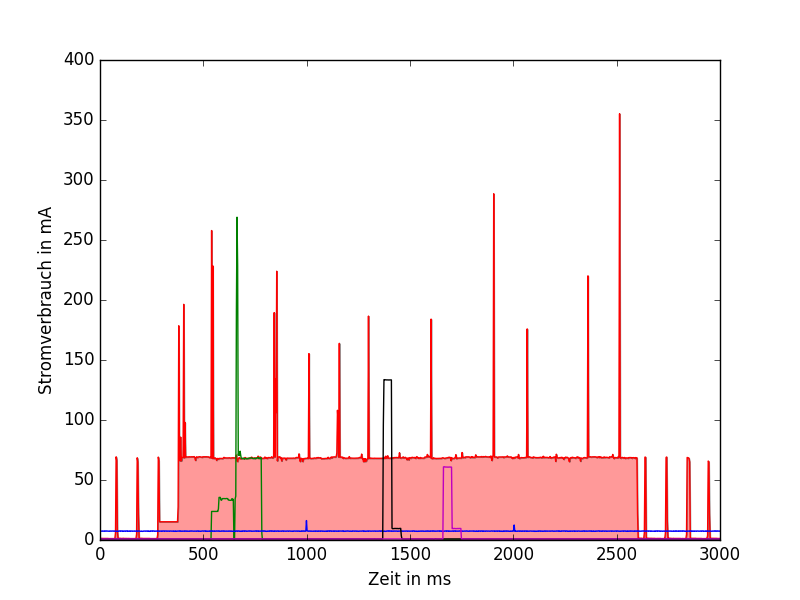
\includegraphics[width=\textwidth]{plots/alle.png}
  \caption{Stromverbrauchskurven für den Ortungsvorgang im Vergleich. Rot: \emph{WiFi-LLS}; Grün: \emph{Probe-Request-Lokalisierung}; Blau: \emph{BLE-Advertising}; Schwarz: LoRa 23 dBm; Lila: LoRa 5 dBm.}
  \label{fig:alle}
\end{figure}


\section{Auswertung}
Es wurden mobile Einheiten mit IEEE 802.11, Bluetooth Low Energy (BLE) und Long Range (LoRa) implementiert und bezüglich ihrer Reichweite und ihres Energieverbrauchs untersucht.

IEEE 802.11 ist den anderen Protokollen weder bei der Reichweite, noch beim Energieverbrauch überlegen. 
Sein Vorteil liegt in der Verfügbarkeit von WLAN \emph{Access Points} (APs), welche als Basisstationen verwendet werden können.
IEEE 802.11 hat jedoch im gegebenen Szenario für den Tunnelbau Probleme mit Bereichen, die durch das WLAN-Netzwerk nicht abgedeckt sind. 
Diese können vermieden werden, wenn spezielle Funktionen beim AP vorausgesetzt werden können.

BLE zeichnet sich durch einen niedrigen Energieverbrauch pro Sendevorgang aus, allerdings zeigte sich bei der Prüfung der Reichweite von BLE auch, dass diese mit 14 bis 32 m nicht sehr groß ist.
Dies wirkt sich negativ auf die Erkennungszuverlässigkeit bei Bereichswechseln aus, außerdem gibt es dadurch große Bereiche, in denen die mobilen Einheiten nicht geortet werden können.

Dieses Problem hat LoRa nicht. 
Seine enorme Reichweite von bis zu 1250 m erlaubt es, dass eine mobile Einheit an jedem Punkt im Tunnel von mehreren Basisstationen geortet werden kann.
Diese Eigenschaft macht die mobile Einheit mit LoRa zu einer sehr zuverlässigen Einheit für die Ortung.
Beachtet werden muss jedoch, dass LoRa Kollisionen nur durch die zufällige Wahl des Kanals zu verhindern versucht.
Es muss daher mit gelegentlichen Kollisionen gerechnet werden.
Daher sollte das Sendeintervall auf die Hälfte des gewünschten Ortungsintervalls gesetzt werden, um eine zuverlässige Ortung im Ortungsintervall zu erreichen.

Aufgrund seiner hohen Reichweite und daraus resultierenden lückenlosen Ortung der mobilen Einheiten, schlägt diese Arbeit LoRa für \emph{zuverlässige funkbasierte Bereichsortung im Tunnelbau} vor.





